\section{Results and discussion}\label{sec:result}
We will now first take a look at the case of two electrons in a potential with different oscillator energies. In order to do so, we preform a Variational Monte Carlo simluation and use the Metropolis algorithm explained in section~\ref{sec:metropolis} to find the energy of the ground state. Therefore we use numerical derivation. We will later introduce analytical calculations based on closed-form expressions as well (section~\ref{sec:analytical}). Besides, we put emphasis on the correlations introduced by the Jastro factor by computing the kinetic and potential energy of the ground state for different oscillator frequencies.\\
In addition we introduce importance sampling and analyse the dependency of the results to the time step $\delta t$.\\
\subsection{Two electron case}\label{sec:2electron}
Since it is the easiest case, we first look at two electrons in a quantum dot interacting with each other. According to \cite{lohne2011} the corresponding energy is at $E = 3~\mathrm{a.u.}$ (atomic units).\\
For the computation we use the variational wave function
\begin{equation}
\psi_T(\mathbf{r_1,r_2}) = C \exp\left[-\alpha\frac{\omega}{2} (r_1^2+r_2^2)\right] \exp \left[ \frac{a_{12} r_{12}}{(1+\beta r_{12})} \right],
\end{equation}
where we start by considering a wide range of $\alpha \in[0.7,1.3]$ and $\beta \in[0.2,0.6]$ first and preform a more precise simulation afterwards. The goal is to find the variational parameters $\alpha$ and $\beta$, where the energy is at its minimum. After the first simulation we notice, that the minimum must be somewhere around $\alpha \in[0.9,1.1]$ and $\beta \in[0.35,0.45]$. This is why we preform a simulation with these boundaries and use 3 000 000 Metropolis cycles to get an accurate result. In figure~\ref{fig:2electron} the energy is plotted depending on both variational parameters $\alpha$ and $\beta$. The 3D-plot results in a bended plane resembling to the shape of a valley. For increasing $\alpha$ the corresponding $\beta$ at minimal energy is decreasing. The minimum energy calculated is 
\begin{align}
E &= 3.0003~\mathrm{a.u.}
\intertext{at}
\alpha &= 0.9867,\\
\beta &= 0.4033.
\end{align}
As mentioned before we were expecting the energy to be at $E=3~\mathrm{a.u.}$, so the calculated value matches the expected one very well. In figure~\ref{fig:2electron} there are some areas, where the plane is not as smooth as in others. We classify these small perturbations to the valley as numerical fluctuations and consider them to be stronly important.\\
To get a better understanding of the influence the parameters have on the calculated energy, figure~\ref{fig:2electronalpha} shows the energy's $\alpha$-dependency for different $\beta$. Consistent with figure~\ref{fig:2electron} this figure reveals, that $\beta$ is shifted depending on $\alpha$ and that $\alpha$ has a larger influence on the energy than the other variational parameter. The errors plotted in figure~\ref{fig:2electronalpha} are almost invisible, since they are very small compared to the energy fluctuations at varying $\alpha$ and $\beta$. There are not many cases, where the error is significantly high, so we consider our results to be of sufficient accuracy.
\begin{figure}[htbp]
    \centering
    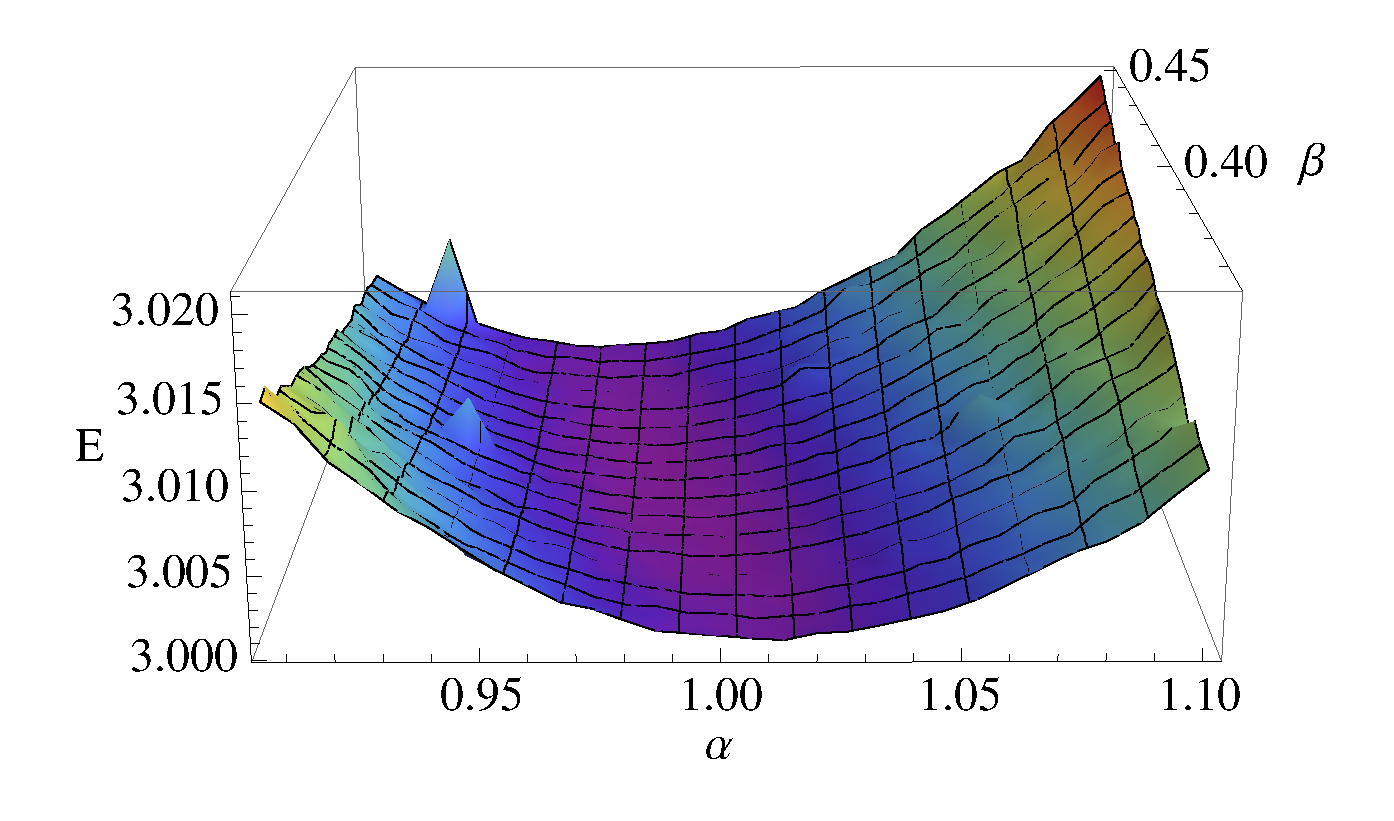
\includegraphics[scale=0.6]{2electron}
    \caption{Plot of $\alpha$- and $\beta$-dependencies of the ground state energy for two interacting electrons at the ground state based on a simulation involving 3 000 000 Metropolis cycles}
    \label{fig:2electron}
\end{figure}
\begin{figure}[htbp]
    \centering
    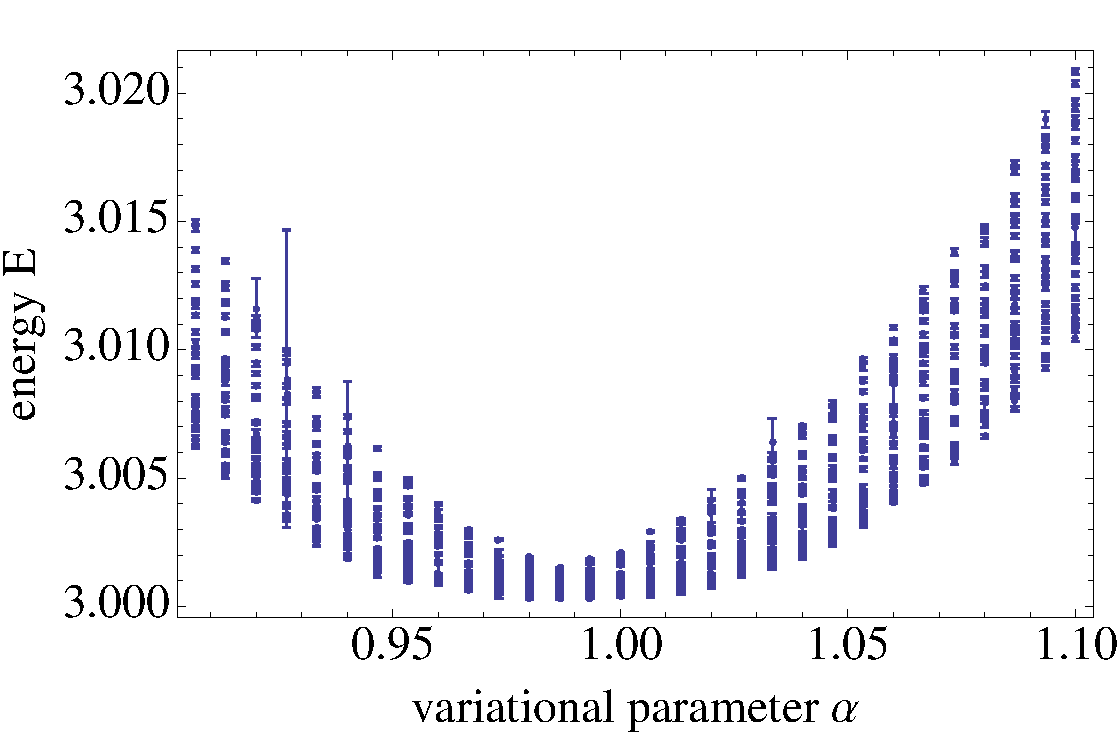
\includegraphics[scale=0.6]{2electronalpha}
    \caption{Plot of $\alpha$-dependency of the ground state energy for two interacting electrons at the ground state for different $\beta$ based on a simulation involving 3 000 000 Metropolis cycles}
    \label{fig:2electronalpha}
\end{figure}
\FloatBarrier
\subsubsection{Jastrow factor}
After computing the ground state energy we now analyse the changement in energy arising from different osciallator potentials $\omega$. The results for $\omega =\{1,0.28,0.01\}$ are shown in table~\ref{tab:omega}. It can be observed, that for small oscillator frequency the kinetic energy drops relative to the total energy of the system. The reason for this is, that for small $\omega$ the potential gets wider, but flatter as well. In this case, the electrons interact less with each other, which results in decreasing kinetic energy.\\
\begin{table}[H]
\centering
\caption{Kinetic and potential energy depending on the oscillator frequency $\omega$}
\begin{tabular}{c|cc|cc}
$\omega$ & $E_{kin} \mathrm{(a.u.)} $& $E_{pot} \mathrm{(a.u.)}$ & $E_{kin}/E \mathrm{(\%)}$ & $E_{pot}/E \mathrm{(\%)}$ \\ \hline
1.00    & 0.8891  & 2.111  & 29.6 & 70.4 \\
0.28 & 0.2616  & 0.774  & 25.3 & 74.7 \\
0.01 & 0.0106 & 0.096 & 9.9 & 90.1
\end{tabular}
\label{tab:omega}
\end{table}
In the wave equation
\begin{equation}
\psi_T(\mathbf{r_1,r_2}) = C \exp\left[-\alpha\frac{\omega}{2} (r_1^2+r_2^2)\right] \exp \left[ \frac{a_{12} r_{12}}{(1+\beta r_{12})} \right]
\end{equation}
only the first exponential term is affected by the oscillator frequency $\omega$, while the Jastro factor does not contain the frequency.\\
For vanishing potential as for $\omega =0.01$ the wave function becomes:
\begin{equation}
\lim_{\omega\rightarrow 0} \psi_T(\mathbf{r_1,r_2}) = C \exp \left[ \frac{a_{12} r_{12}}{(1+\beta r_{12})} \right] = C J,
\end{equation}
where $J$ is the Jastrow factor. This means, that in this case the Jastrow factor adopts a more important role. The correlations introduced by the Jastro factor ...
\subsubsection{Importance sampling: $\delta t$-dependency}
To obtain accurate results we also introduce important sampling and optimize the calculation of the energy by studying its time step dependency. We will refer to the time step as $\delta t$. The time step plays an important role in importance sampling, since it the biasing when calculation new random numbers. For large $\delta t$ the newly picked random numbers for the particle position can vary more, than for smaller $\delta t$. It is therefore relevant to use a reasonable time step to aviod jumping to far in the position or to get stuck in one place as explained previously in section~\ref{sec:importance}. In figure~\ref{fig:importance} we plotted the energy calculated for $\alpha = 0.98$ and $\beta = 0.40$ (according to~\ref{sec:2electron}) for diverse $\delta t$. Comparing the results including importance sampling to those in section~\ref{sec:2electron} we notice, that with importance sampling we can obtain a lot smaller energies, than when using a brute force Metropolis algorithm. This shows, that the importance sampling has an impact on the precision of the results, because we get energies very near the exact solution.\\
Concerning the optimal value of $\delta t$, it is obvious in figure~\ref{fig:importance}, that it must be $\delta t \in [0.1,0.2]$. Because of the statistical spread of the energy values, we cannot find the one and only perfect $\delta t$-value. For large time steps the energy converges to $E=3.0016$ ...
%Gleicher Wert wie in Aufgabenteil b)?
\begin{figure}[htbp]
    \centering
    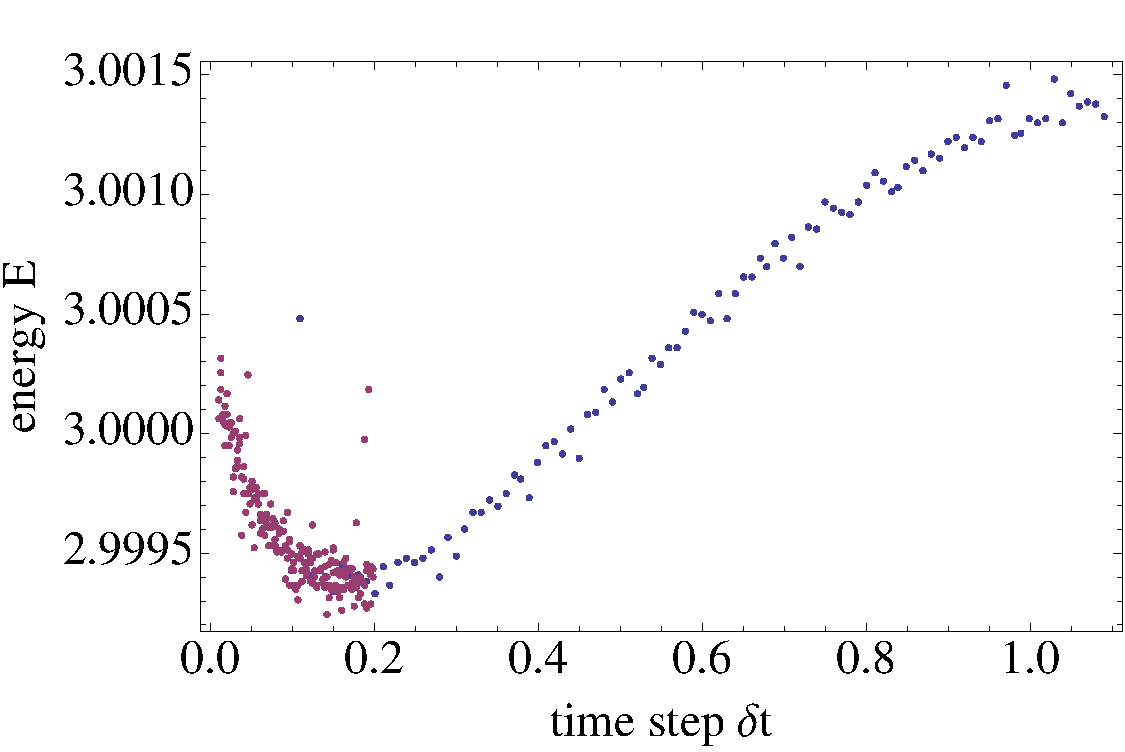
\includegraphics[scale=0.6]{importance}
    \caption{Results of energy calculation for varying time steps $\delta t$ in the importance sampling. The blue dots refer to a wide-spaced simulation for $\delta t \in [0.1,1]$ with step length $\Delta (\delta t) = 0.01$, whereas the violet dots refer to $\delta t\in [0.01,0.2]$ with $\Delta(\delta t) = 0.001$}
    \label{fig:importance}
\end{figure}
\FloatBarrier

\subsection{Six electron case}

\subsubsection{Virial theorem}
\subsection{Analytical Calculations}\label{sec:analytical}